\chapter**{Introdução}
\enlargethispage{.5\baselineskip}
Nos dias atuais, um problema latente para a agricultura mundial é a perda da produção devido à problemas com pragas. De acordo com a Organização das Nações Unidas para a Alimentação e a Agricultura (FAO), todo ano, entre 20 e 40\% da produção agrícola é perdida em função desses problemas \citep{FAO:2021}. Levando tal fato em consideração, é evidente a importância de se diagnosticar doenças em plantas de maneiras que sejam tanto eficientes quanto baratas, visando a minimização dos danos oriundos das pragas na agricultura mundial.

A detecção e diagnóstico de doenças em plantas pode ser feita por inspeção visual, avaliação microscópica de características morfológicas, ou ainda técnicas moleculares, sorológicas ou microbiológicas~\citep{Mahlein:2016}.
Todas essas formas de análise são baseadas em tecnologias ou conhecimentos específicos, sendo portanto altamente dependentes de pessoal qualificado e especialista.
Esse processo, além de ser feito em escala reduzida, é custoso e complexo, o que demonstra a necessidade de inovações tecnológicas que auxiliem nesta tarefa e a tornem mais simples e acessível para aqueles que desenvolvem atividades agrícolas. 

Paralelamente à essa necessidade, podemos observar avanços tecnológicos substanciais que vêm sendo feitos no desenvolvimento de tarefas complexas como a criação de agentes conversacionais \citep{LLMsScience, Minaee:2024} e direção autônoma \citep{Badue2019Self-Driving}, por exemplo.

Assim, é considerável que o acúmulo científico que a humanidade alcançou nos últimos anos (evidenciado pelos avanços tecnológicos comentados) possibilite a construção de inovações tecnológicas que auxiliem os produtores rurais contra esse problema latente.

Na realidade, essa consideração se mostra realista. O artigo de~\cite{Mahlein:2016} discute o uso de técnicas de imageamento em agricultura, destacando a questão de detecção de doenças em plantas. O trabalho lista sensores convencionais que geram imagem RGB, câmeras multi ou hiper-espectrais, sensores termais, sensores de fluorescência, e outros sensores capazes de medir biomassa e outras características estruturais das plantas. Dentre essas tecnologias, câmeras convencionais que geram imagens RGB estão amplamente  disponíveis, são portáteis e de fácil manuseio, principalmente em \emph{smartphones}. Assim, o processamento computacional dessas imagens poderia ajudar na identificação precoce dessas doenças e, por conseguinte, diminuir as perdas envolvidas.

A percepção que técnicas de visão computacional podem ajudar nesse problema não é algo novo. No cenário nacional, recentemente a Embrapa\footnote{\url{https://www.embrapa.br/}} publicou uma matéria intitulada \href{https://www.embrapa.br/busca-de-noticias/-/noticia/78204383/inteligencia-artificial-identifica-plantas-doentes-simulando-processo-cerebral}{``Inteligência artificial identifica plantas doentes simulando processo cerebral''} na qual é discutida uma parceria estabelecida por ela com empresas privadas para desenvolver inovações na detecção automática de doenças em plantas. Além disso, embora aplicativos de celular voltados para a identificação de doenças em plantas estejam se tornando mais comuns, ainda enfrentam críticas devido à sua baixa precisão e limitações funcionais \citep{Siddiqua2022}


\section**{Motivação}
\label{sec:motivação}
A partir de uma perspectiva acadêmica, os recentes avanços na área de Visão Computacional, devido ao contínuo melhoramento das técnicas de \emph{deep learning}~\citep{Goodfellow-et-al-2016}, tornaram possíveis trabalhos sobre detecção de doenças em imagens de plantas que fazem uso de modelos de redes neurais profundas. Entre esses trabalhos, a maioria considera imagens de folhas de plantas obtidas utilizando-se câmeras convencionais e trata do problema de classificação de doenças~\citep{Singh:2017,Mohanty:2016,Geetharamani2019,plantxvit}. 

Essas técnicas de \emph{deep learning} são baseadas em redes neurais~\citep{Nielsen:2015,Goodfellow-et-al-2016} que possuem a capacidade de processar dados em seu formato bruto e extrair automaticamente as representações (características) que são mais eficazes para a inferência final esperada. Essa capacidade, resultante do processo de treinamento da rede neural, faz com que os métodos sejam facilmente adaptados para imagens com diferentes características. Assim, o desenvolvimento de soluções para novos cenários de aplicação --- como culturas diferentes e imagens com características diferentes ---  é bastante agilizado, o que reforça o potencial dessa abordagem. 

O conjunto de dados público mais utilizado para o treinamento e avaliação dos modelos de visão computacional para detecção de doenças em plantas (e dos trabalhos supracitados) é o \emph{PlantVillage dataset}~\citep{HughesS15, Yao2023}. Exemplos de imagens desse \emph{dataset} são mostrados na figura~\ref{fig:samples}.

\begin{figure}[hbt!]
  \centering
  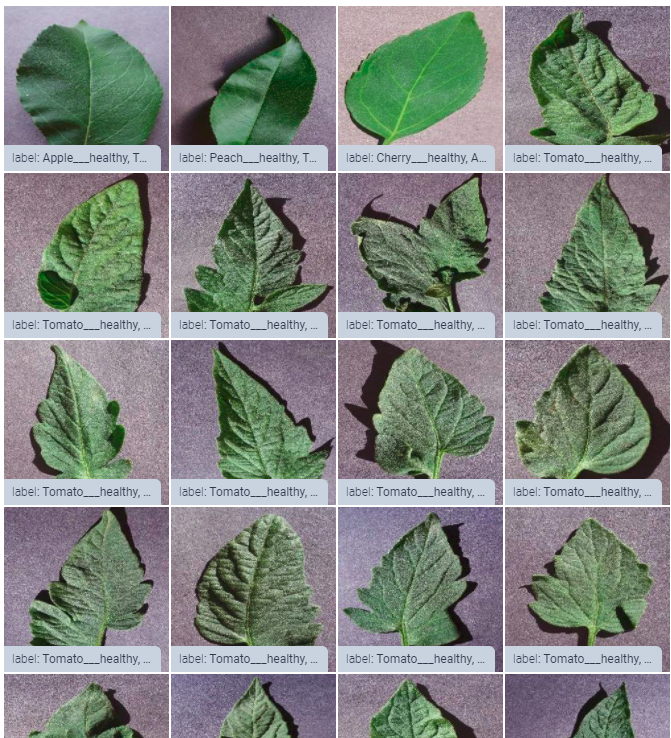
\includegraphics[width=0.8\linewidth]{images/plantvillage.png}
  \caption{\label{fig:samples}Exemplos de imagens de folhas no \emph{dataset} \emph{PlantVillage} (extraído de \url{https://paperswithcode.com/dataset/plantvillage}).}
\end{figure}

Contudo, infelizmente uma série de questões relacionadas à qualidade dos dados do \emph{PlantVillage} faz com que os ótimos resultados demonstrados nos trabalhos acadêmicos em questão não se traduzam para o contexto do cotidiano dos agricultores. Seja pela natureza das imagens, compostas de folhas de plantas em um plano de fundo de cor sólida e sem grandes variações na iluminação (o que não é reproduzido em fotos tiradas no campo) \citep{Yao2023, HughesS15, Singh:2017, Coletta2022Optimal} ou por problemas referentes à condições de captura (balanço de branco, exposição, foco) e padrões observados nos planos de fundo das imagens que se constituem como atributos que têm correlações espúrias com o rótulo das imagens e, por isso, acabam por facilitar muito a tarefa do modelo classificador desenvolvido \citep{Noyan:2022}.

Como comentado, a consequência desses vieses é que, apesar de artigos corriqueiramente publicados obterem resultados muito impressionantes na tarefa de classificação de doenças de plantas, esses resultados não se generalizam para situações reais e, portanto, nos dão uma falsa ideia de que o problema de classificação de doenças de plantas utilizando visão computacional já está resolvido. Isso acaba por ter o resultado oposto do esperado, atrasando o desenvolvimento tecnológico e científico.

Dessa forma, fica evidente que é necessário investir em alternativas para o desenvolvimento de conjunto de dados abertos, robustos e que tenham passado por curadoria. Somente assim avançaremos no desenvolvimento de modelos de visão computacional aplicados à detecção de doenças em plantas, com resultados que realmente farão a diferença no dia a dia dos agricultores que se beneficiariam dessas ferramentas abertas e acessíveis. Essa é a principal motivação desse trabalho de formatura supervisionado.

\section**{Objetivo}
O objetivo deste trabalho é desenvolver um sistema que possibilite a produção de melhores conjuntos de dados de visão computacional no domínio da agricultura. Para isso, a ideia proposta é a implementação de um sistema em que os usuários possam enviar fotos de, por exemplo, folhas de plantas doentes, para obter o diagnóstico da doença pelo sistema. As imagens enviadas pelos usuários serão acumuladas em um banco de dados de imagens e posteriormente revisadas por usuários especialistas, que poderão corrigir os diagnósticos feitos pelo sistema. Depois disso, as imagens revisadas passam a fazer parte de um novo conjunto de dados, que será incrementado com o tempo com as imagens enviadas para a plataforma. Dessa forma, consideramos que será possível produzir conjuntos de dados de boa qualidade e volume de maneira colaborativa.
